\documentclass{beamer}
\usepackage[T1]{fontenc}
\usepackage[utf8]{inputenc}
\usepackage[english]{babel}
\usepackage{listings}
\title{C written DBMS}
\author[Tecchia, Ritter]{Lorenzo Tecchia, Nathan Ritter \\
\texttt{lorenzot@zedat.fu-berlin.de} \\
\texttt{rittern@zedat.fu-berlin.de}}
\institute[FU Berlin]{Freie Universität Berlin}
\logo{
\includegraphics[width=0.13\textwidth]{FUlogo.png}}
\usetheme{Berkeley}
\begin{document}

\begin{frame}
	\maketitle
\end{frame}

\begin{frame}
	\frametitle{Overview of the presentation}
	\tableofcontents
\end{frame}

\section{Introdcution}
\begin{frame}
	\frametitle{DBMS Idea}
	\begin{columns}
	\begin{column}{0.4\textwidth}	
		Our Project is a DBMS written in the C Language. \\ Even tho the C language is a very old language it's still widely used nowadays, to write many DBMSs.
	\end{column}
	
	\begin{column}{0.4\textwidth}

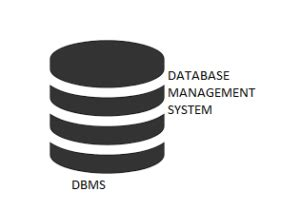
\includegraphics[width=1.4\columnwidth]{th-1536893874.jpg}			
	
	\end{column}

	\end{columns}
\end{frame}

\begin{frame}
	\frametitle{What is a DBMS}
	\begin{columns}
	\begin{column}{0.4\textwidth}
		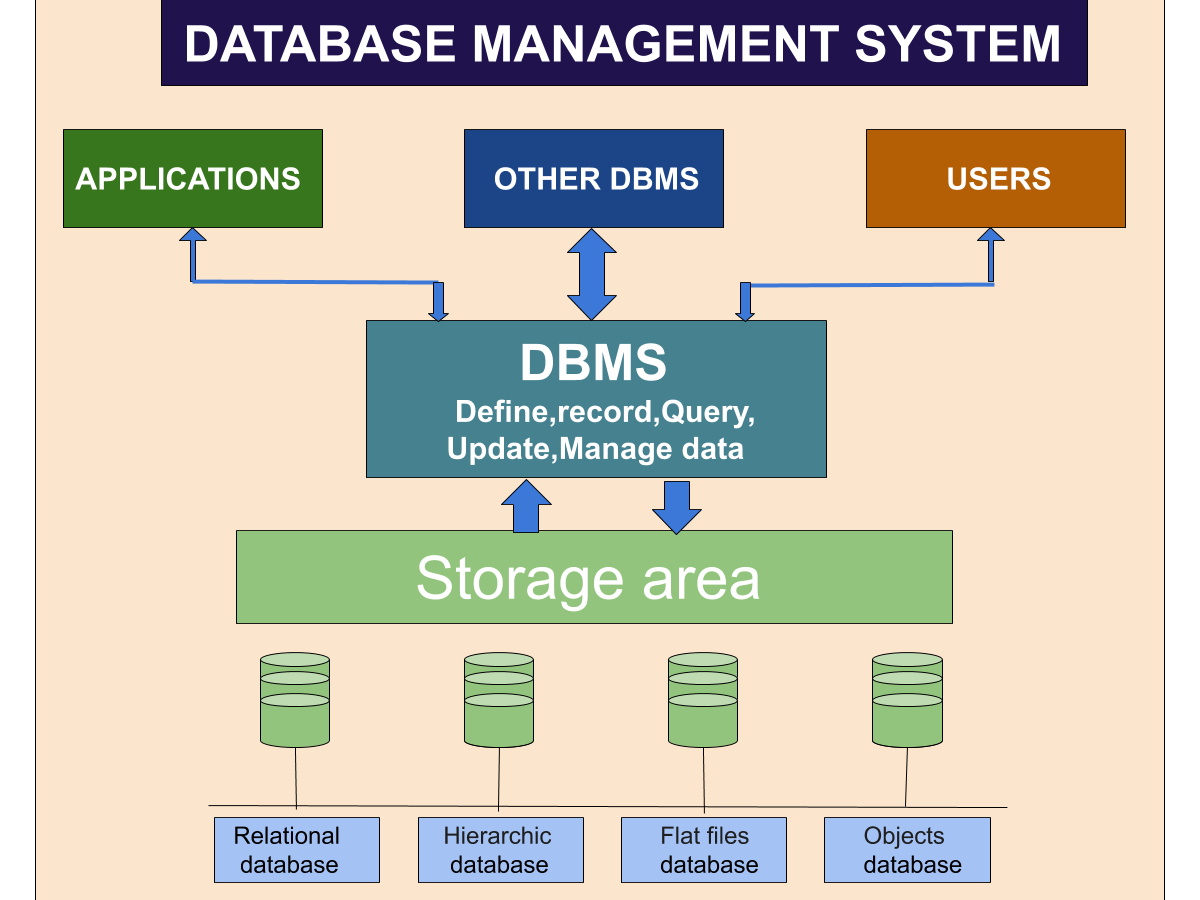
\includegraphics[width=1.2\columnwidth]{/Users/lorenzotecchia/Documents/ESAMI/SoftwareEngineering/SoftwareEngineeringAssignments/SoftwareEngineering_LaTeX/Assignments/A-2/Presentation/DBMS-database-management-systems-3193913233.png}
	\end{column}
	
	\begin{column}{0.4\textwidth}
	\begin{itemize}
		\item DBMS stands for Database Management system. 
		\item A DBMS is a tool for storing retrieving stored data.
		\item DMBS are needed anywhere you have a data.		
	\end{itemize}
			 
	\end{column}
	
	\end{columns}


\end{frame}

\section{Domain and Requirements}
\begin{frame}
	\frametitle{Functions of a DBMS}
	\begin{itemize}
		\item So what would be the basics functions of a DBMS?
		\item What are the most crucial capabilities of any modern DBMS?
	\end{itemize}
	  (Security, Library management, server management, Type definition, ecc...)
\end{frame}

\begin{frame}
	\frametitle{Libraries for string management}
	\begin{columns}
	\begin{column}{0.4\textwidth}
		PostgreSQL has the REGEX library, but our software could have any ad hoc library that the customer requires. 		
	\end{column}
	
	\begin{column}{0.4\textwidth}
		
\includegraphics[width=\columnwidth]{regex1-985818275.png}
	\end{column}

	\end{columns}


\end{frame}

\begin{frame}
	\frametitle{Able to manage different users}
	\begin{columns}
	\begin{column}{0.4\textwidth}
		Different users with different access policy would have to be managed by the DBMS and would have the ability to group them accordingly.

	\end{column}
	\begin{column}{0.4\textwidth}
		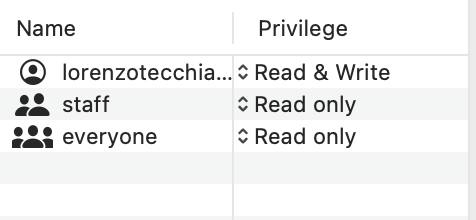
\includegraphics[width=\columnwidth]{rootaccess.png}

	\end{column}
	\end{columns}
\end{frame}

\begin{frame}
	\frametitle{Able to manage different servers}
	\begin{columns}
	\begin{column}{0.4\textwidth}
	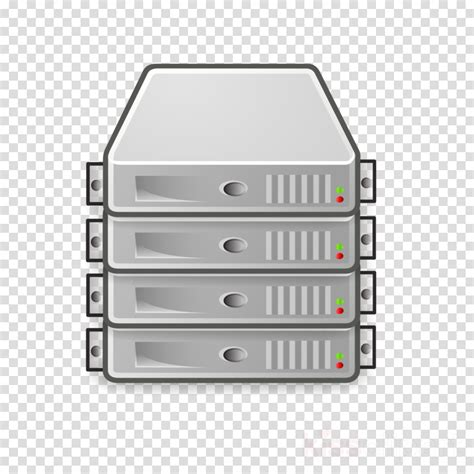
\includegraphics[width=\columnwidth]{serverimage.jpg}
			\end{column}
	\begin{column}{0.4\textwidth}
	Different users would have many servers between them, so the DBMS should be able to switch between them.	
	\end{column}

	\end{columns}

	
\end{frame}

\begin{frame}
	\frametitle{Different data types}
	\begin{columns}
	\begin{column}{0.4\textwidth}
		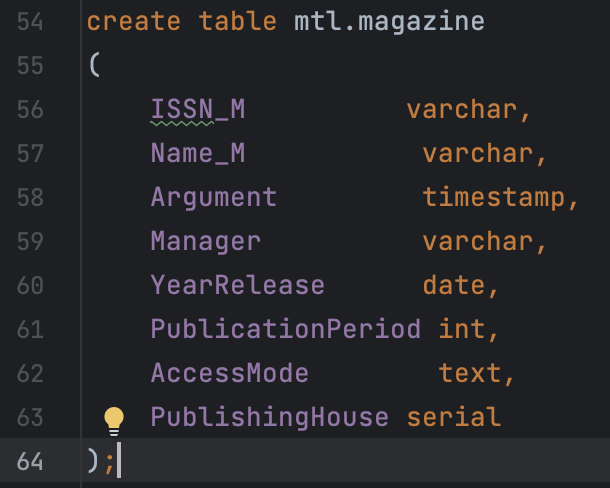
\includegraphics[width=\columnwidth]{tablecreation2.png}
	\end{column}
		\begin{column}{0.4\textwidth}
	Tables of RDBMSs (Relational DBMSs) would have different attributes and so the need for different data types.
	\end{column}
		\end{columns}
\end{frame}

\begin{frame}
	\frametitle{Create Indexes}	
	\begin{columns}
	\begin{column}{0.4\textwidth}
		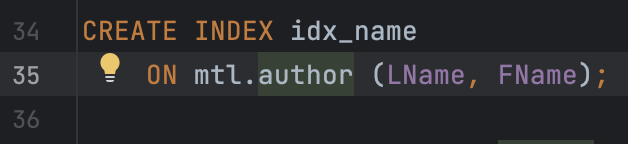
\includegraphics[width=\columnwidth]{indexcreation.png}
	\end{column}
		\begin{column}{0.4\textwidth}
	Indexes are necessary for fast data retrieval and data parsing. Like primary keys, or the so called indexes. 
	\end{column}
	\end{columns}
\end{frame}

\begin{frame}
	\frametitle{Security}
	User shall have passwords to log into their servers, and to make changes to the data itself.
\end{frame}


\begin{frame}
	\frametitle{Data retrieval time}	
	\begin{columns}
	\begin{column}{0.4\textwidth}
		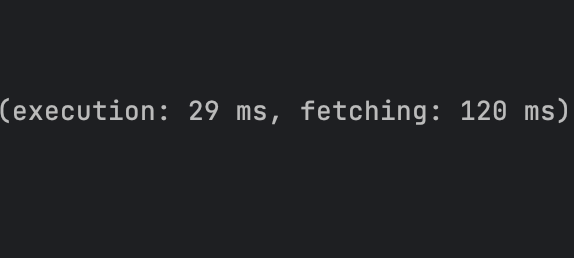
\includegraphics[width=\columnwidth]{elapsedtime.png}
	\end{column}	
	\begin{column}{0.4\textwidth}
	The DBMS should provide functions to monitor the time elapsed for every query done the the servers. And provide any ad-hoc required speed/performance. 
	\end{column}
	\end{columns}
\end{frame}

\begin{frame}
	\frametitle{Accuracy}	
	Data accuracy means providing capabilities or functions that refer to error-free records that can be used as a reliable source of information.(e.g. not allowing negative numbers for item counting).
\end{frame}

\begin{frame}
	\frametitle{Consistency}	
	In database systems, consistency (or correctness) refers to the requirement that any given database transaction must change affected data only in allowed ways. (e.g. constraints, cascades, triggers)
\end{frame}

\section{Target Group of the software}
\begin{frame}
	\frametitle{Target Groups of our Software}	
	\centering What are the target group of the software?
\end{frame}

\begin{frame}
	\frametitle{Programmers}	
	\begin{columns}
	\begin{column}{0.4\textwidth}
		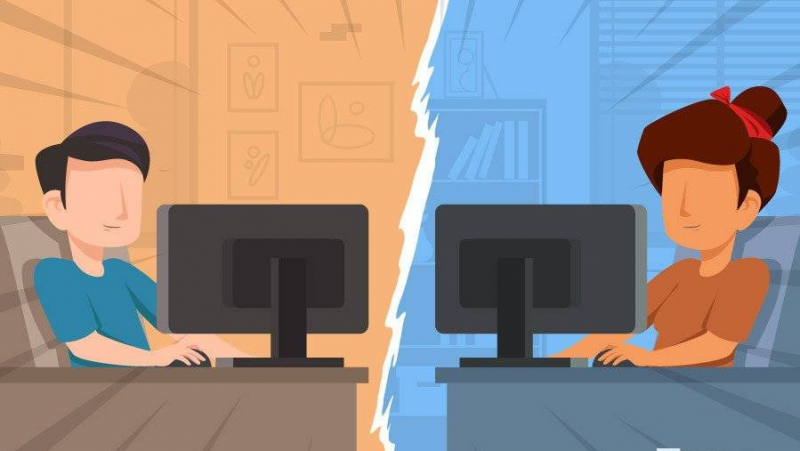
\includegraphics[width=\textwidth]{developer.png}
	\end{column}	
	\begin{column}{0.4\textwidth}
	Programmers developing Applications/Systems etc. for companies that need to store large amounts of data efficiently and effectively 
	\end{column}
	\end{columns}
	
\end{frame}

\begin{frame}
	\frametitle{Customers}
	\begin{columns}
	\begin{column}{0.4\textwidth}
			What are Our potential Customers? \\ Well Everyone with an incline for programming and Knowledge of Databases
	\end{column}
		\begin{column}{0.4\textwidth} 	
		
\includegraphics[width=\columnwidth]{programmingphoto.png}
		\end{column}
		\end{columns}
\end{frame}

\begin{frame}
	\frametitle{Companies}	
	Could shape out the DBMS to their needs, or request specifics functionalities that perfectly meet their needs and requirements. 
\end{frame}

\section{Knowledge level required}
\begin{frame}
	\frametitle{What level of knowledge is requires to use the software?}
	Having deeper knowledge of DBMSs will be useful, to provide clever solutions for the same problem, but even newbies can approach the software.
\end{frame}

\section{Software drawbacks}
\begin{frame}
	\frametitle{Problems with our software}
	\begin{columns}
	\begin{column}{0.4\textwidth}
	 What problems will we face? \\ Lots of other DBMS are available and well established, like PostgreSQL or SQLite. (Which are also written in C).		
	\end{column}
		\begin{column}{0.4\textwidth}
		
\includegraphics[width=\columnwidth]{sqlitelogo.jpg}
	 \end{column}
	 \end{columns}
\end{frame}

\begin{frame}
	\frametitle{Adaptation/Migration}
	\begin{columns}
	\begin{column}{0.4\textwidth}
		
\includegraphics[width=1.4\columnwidth]{postgelogo.png}
	\end{column}
		\begin{column}{0.4\textwidth}
	Changing the DBMS for and existing Database is a very complex process so, companies wouldn't be totally inclined to change to our software(if the already have their own).	
	\end{column}
		\end{columns}
\end{frame}

\begin{frame}
	\frametitle{The End}
	\begin{center}
		\Huge\textbf{THE END} 
	\end{center} 
\end{frame}

\end{document}
